\documentclass[aspectratio=169]{beamer}

% -------------------------------------------------
% COLORS
% -------------------------------------------------
\usepackage{xcolor}

\definecolor{themeColor}{RGB}{33,26,82}

\definecolor{color1}{HTML}{3AB795} % greenish
\definecolor{color2}{HTML}{48439B} % dark blue
\definecolor{color3}{HTML}{AB74CF} % purple
\definecolor{color4}{HTML}{CA697C} % pinkish
\definecolor{color5}{HTML}{F8B100} % orange

% -------------------------------------------------
% THEME CUSTOMIZATION
% -------------------------------------------------
\setbeamercolor{structure}{fg=themeColor}
\setbeamercolor{frametitle}{fg=white,bg=themeColor}
\setbeamercolor{title}{fg=white,bg=themeColor}
\setbeamercolor{block title}{fg=white,bg=color2}
\setbeamercolor{block body}{bg=gray!5}
\setbeamercolor{alerted text}{fg=color3}

\setbeamertemplate{navigation symbols}{}
\setbeamertemplate{footline}[frame number]

% -------------------------------------------------
% PACKAGES
% -------------------------------------------------
\usepackage{amsmath, amssymb}
\usepackage{graphicx}
\usepackage{booktabs}
\usepackage[T1]{fontenc}
\usepackage[utf8]{inputenc} % allow UTF-8 characters in source
\usepackage{lmodern}        % nicer fonts with T1

% -------------------------------------------------
% TITLE INFO
% -------------------------------------------------
\title{Exam Presentation}
\subtitle{Probability Theory, Stochastic Processes and Applied Statistics}
\author{David Redondo}
\date{2026}

% -------------------------------------------------
% SECTION TITLE + MINI TOC   <-- MOVE HERE
% -------------------------------------------------
\AtBeginSection[]
{
  \begin{frame}[plain]
    \vfill
    \centering
    {\usebeamerfont{title}\color{themeColor}\insertsectionhead\par}
    \vspace{1em}
    \begin{minipage}{0.8\textwidth}
      \tableofcontents[currentsection, hideothersubsections]
    \end{minipage}
    \vfill
  \end{frame}
}

% =================================================
\begin{document}
% =================================================

% -------------------------------------------------
\begin{frame}
\titlepage
\end{frame}
% =================================================
\section{Workshop 1: Wind Speed Distributions}
% =================================================
% -------------------------------------------------
\begin{frame}{Motivation}
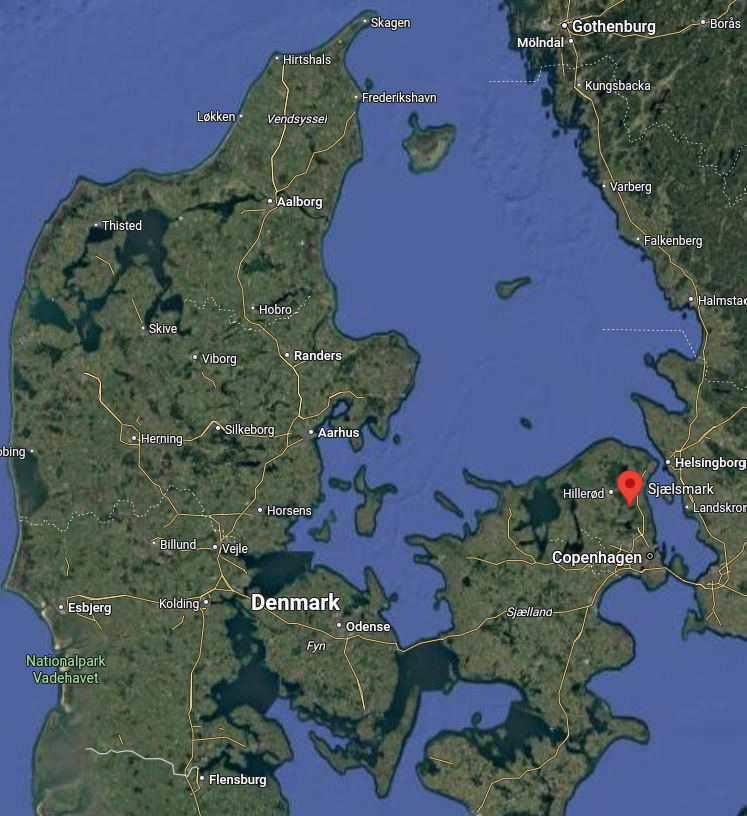
\includegraphics[width = 0.5\textwidth]{wind_location}

\end{frame}

% -------------------------------------------------
\begin{frame}{The Weibull Distribution}
A random variable $X$ follows a Weibull distribution with parameters
$k>0$ (shape) and $\lambda>0$ (scale):

\[
X \sim \text{Weibull}(k,\lambda)
\]

\[
f(x) =
\begin{cases}
\dfrac{k}{\lambda}\left(\dfrac{x}{\lambda}\right)^{k-1}
e^{-(x/\lambda)^k}, & x>0 \\
0, & x \le 0
\end{cases}
\]

\begin{itemize}
  \item $k$ controls the shape
  \item $\lambda$ stretches the distribution
\end{itemize}
\end{frame}

% -------------------------------------------------
\begin{frame}{Distribution Function}
The distribution function is

\[
F(x) = P(X \le x) = \int_{-\infty}^{x} f(x) dx
\]

For the Weibull distribution:
\[
F(x) = 1 - e^{-(x/\lambda)^k}, \quad x>0
\]

\begin{itemize}
  \item Obtained by integrating the density using the substitution $u=(x/\lambda)^k$
\end{itemize}

We can also prove:
\[
\ln\big(-\ln(1-F(x))\big)
= -k\ln(\lambda) + k\ln(x)
\]

\end{frame}

% -------------------------------------------------
\begin{frame}{Mean and Variance}
The mean of a Weibull distributed variable is
\[
\mu = \int_{-\infty}^{\infty} x\cdot F(x) dx
\]
\[
\mu = \lambda \Gamma\!\left(1+\frac{1}{k}\right)
\]
The variance is
\[
\text{Var}(X) = \int_{-\infty}^{\infty} x^2\cdot F(x) dx - \mu^2
\]
\[
\text{Var}(X)
= \lambda^2\left(
\Gamma\!\left(1+\frac{2}{k}\right)
- \Gamma\!\left(1+\frac{1}{k}\right)^2
\right)
\]

\[
\sigma = \lambda
\sqrt{
\Gamma\!\left(1+\frac{2}{k}\right)
- \Gamma\!\left(1+\frac{1}{k}\right)^2
}
\]
\end{frame}

% -------------------------------------------------
\begin{frame}{Wind Speed Data}

First step: visualize the data using a histogram

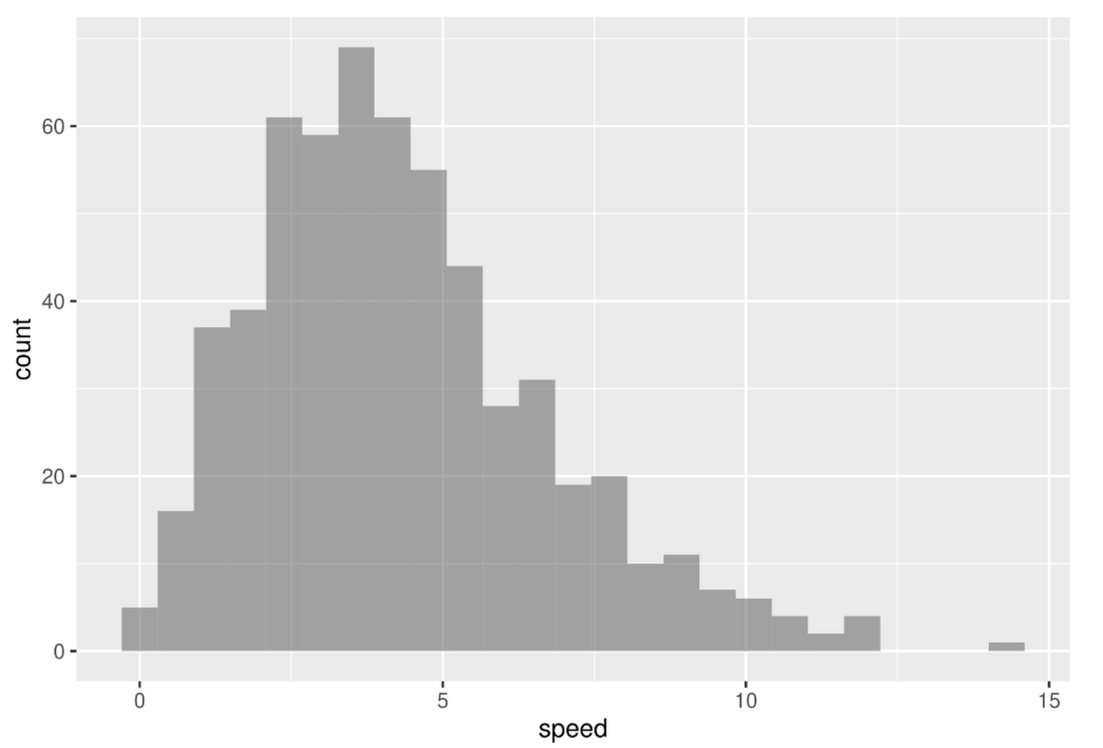
\includegraphics[width = 0.5\textwidth]{wind_histogram}

\begin{itemize}
  \item Wind speed is:
  \begin{itemize}
    \item Positive
    \item Right-skewed
    \item Not normally distributed
  \end{itemize}
\end{itemize}
\end{frame}

% -------------------------------------------------
\begin{frame}{Empirical Distribution Function}
Let the ordered observations be
\[
x_{(1)} \le x_{(2)} \le \dots \le x_{(n)}
\]

For the $i$th ordered value:
\[
F(x_{(i)}) \approx \frac{i}{n}
\]

\begin{itemize}
  \item Exactly $i$ observations are $\le x_{(i)}$
  \item This approximates the true CDF
\end{itemize}
\end{frame}

% -------------------------------------------------
\begin{frame}{Weibull Probability Plot}

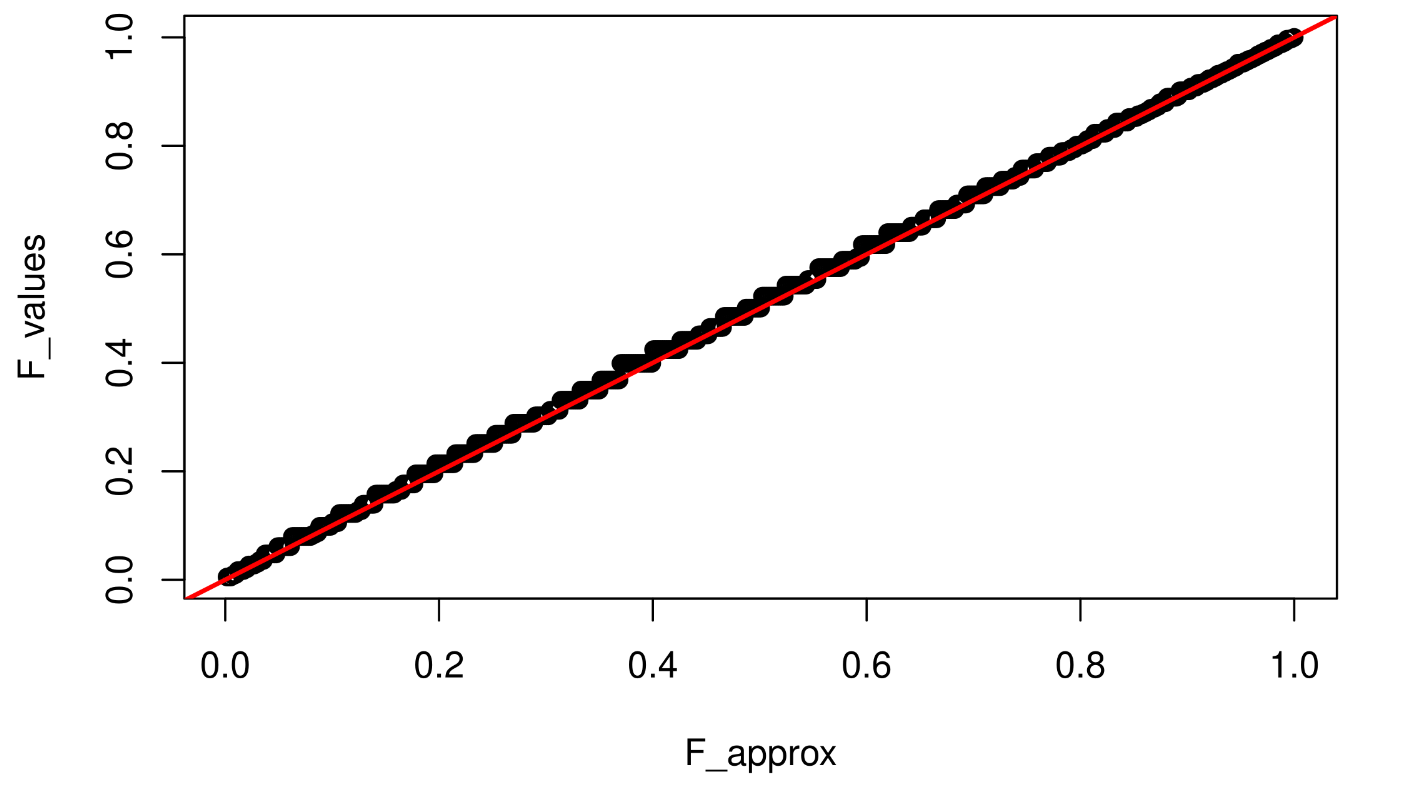
\includegraphics[height = 0.5\textwidth]{wind_yx}

\end{frame}
% -------------------------------------------------
\begin{frame}{Weibull Probability Plot}
Define
\[
u_i = \ln(x_{(i)}), \quad
v_i = \ln\!\left(-\ln\!\left(1-\frac{i}{n}\right)\right)
\]

Remember 
\[
\ln\big(-\ln(1-F(x))\big)
= -k\ln(\lambda) + k\ln(x)
\]

If data follows a Weibull distribution:
\[
v_i \approx -k\ln(\lambda) + k u_i
\]

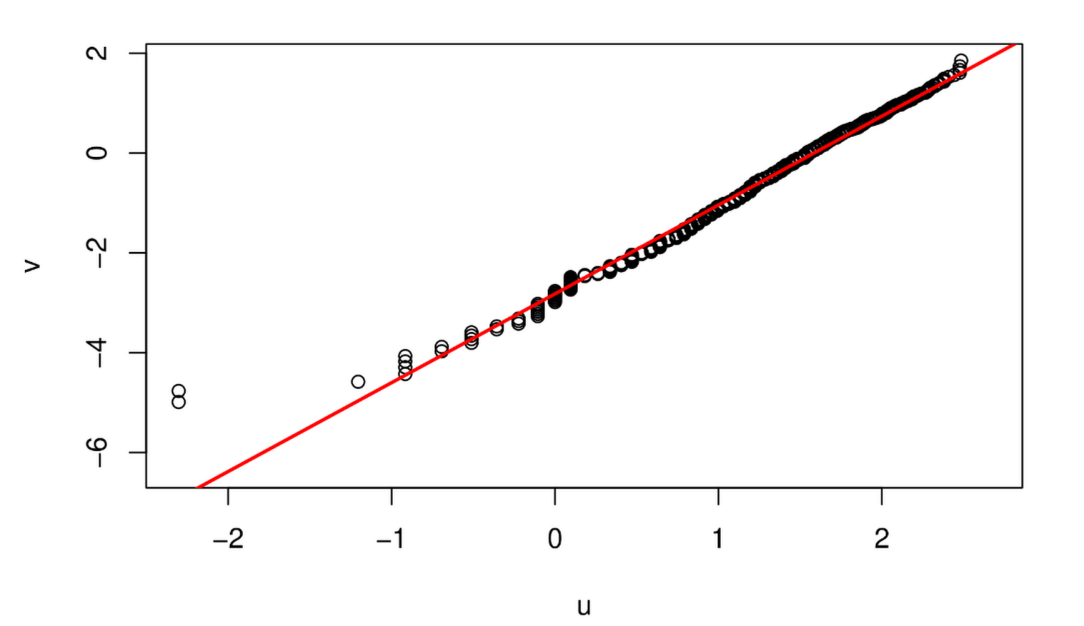
\includegraphics[height = 0.3\textwidth]{wind_weibull_fit}

$k$ and $\lambda$ are calculated from the intercept and slope:
\begin{itemize}
  \item $k = 1.78$
  \item $\lambda = 4.87$
\end{itemize}

\end{frame}

% -------------------------------------------------
\begin{frame}{Weibull Probability Plot}

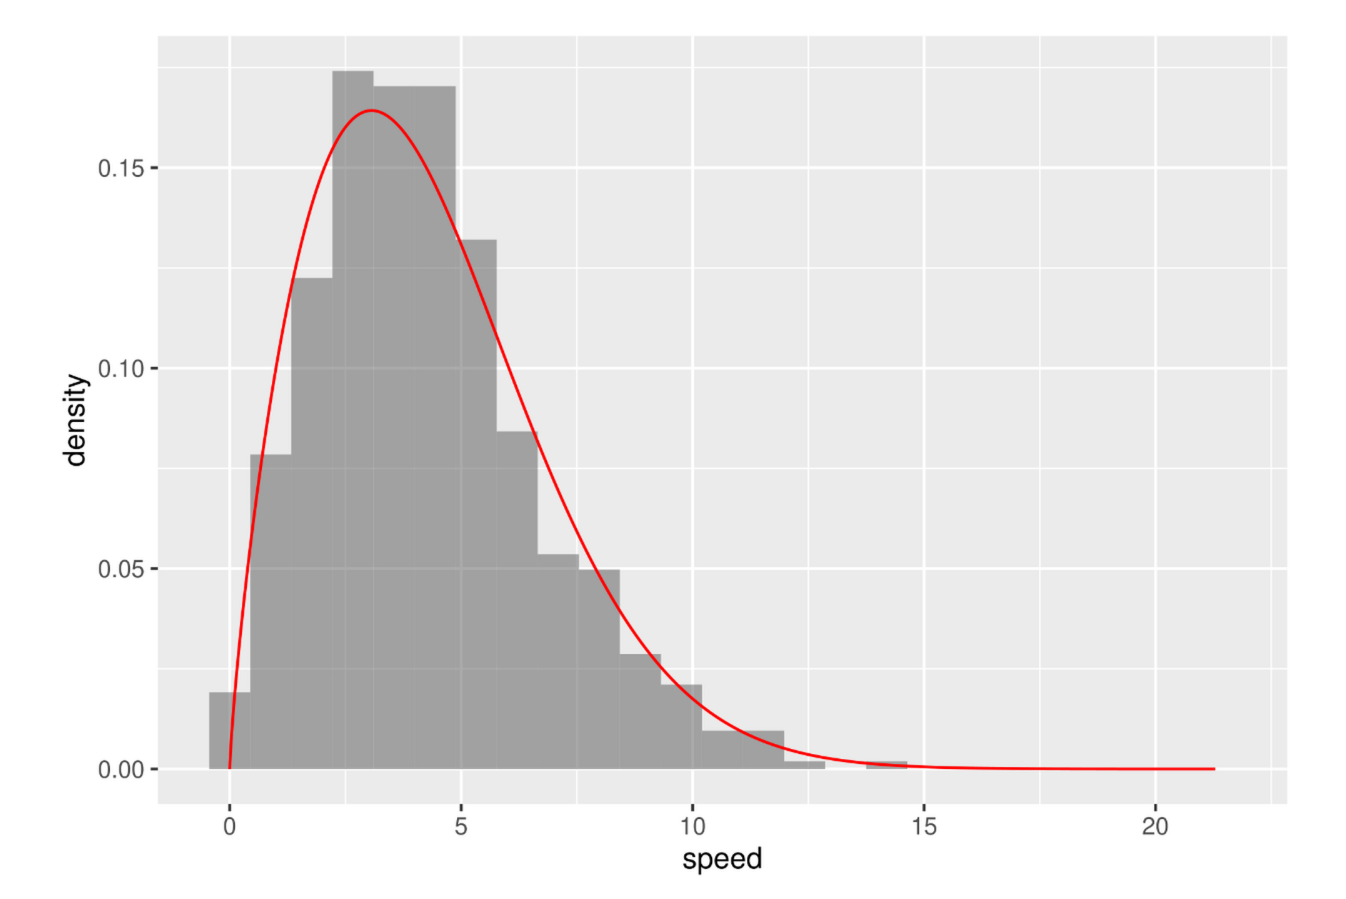
\includegraphics[height = 0.4\textwidth]{wind_weibull_fit_histogram}

$k$ and $\lambda$ are calculated from the intercept and slope:
\begin{itemize}
  \item $k = 1.78$
  \item $\lambda = 4.87$
\end{itemize}

\end{frame}
% -------------------------------------------------
\begin{frame}{Sample Moments and CLT}
Let $X_1,\dots,X_n$ be i.i.d. Weibull variables and
\[
\bar X = \frac{1}{n}\sum_{i=1}^n X_i
\]

By the Central Limit Theorem:
\[
\bar X \approx N\!\left(\mu,\frac{\sigma^2}{n}\right)
\]

for sufficiently large $n$.
\end{frame}
% -------------------------------------------------
\begin{frame}{Sample Moments and CLT}
From before we know:
\[
\mu = \lambda \Gamma\!\left(1+\frac{1}{k}\right)
\]
\[
\sigma = \lambda
\sqrt{
\Gamma\!\left(1+\frac{2}{k}\right)
- \Gamma\!\left(1+\frac{1}{k}\right)^2
}
\]
Evaluating with $k = 1.78$ and $\lambda = 4.87$,

\[
\mu = 4.333 \text{ and } \sigma = 3.766
\]
\end{frame}

% -------------------------------------------------
\begin{frame}{Simulation Study}
\begin{itemize}
  \item Sample size: $n=30$
  \item Repeat sampling 500 times
  \item Store each sample mean
\end{itemize}

\bigskip
We examine:
\begin{itemize}
  \item Mean of sample means
  \item Standard deviation (standard error)
  \item Shape of the distribution
\end{itemize}
\end{frame}

% -------------------------------------------------
\begin{frame}{Results}
\begin{itemize}
  \item Mean of $\bar X$ is close to $\mu$ ($\bar x = 4.326$, $\mu = 4.333$)
  \item Standard deviation is close to $\sigma/\sqrt{n}$ ($SD = 0.490$, $\sigma/\sqrt{n} = 0.688$)
  \item QQ-plot shows approximate normality
\end{itemize}

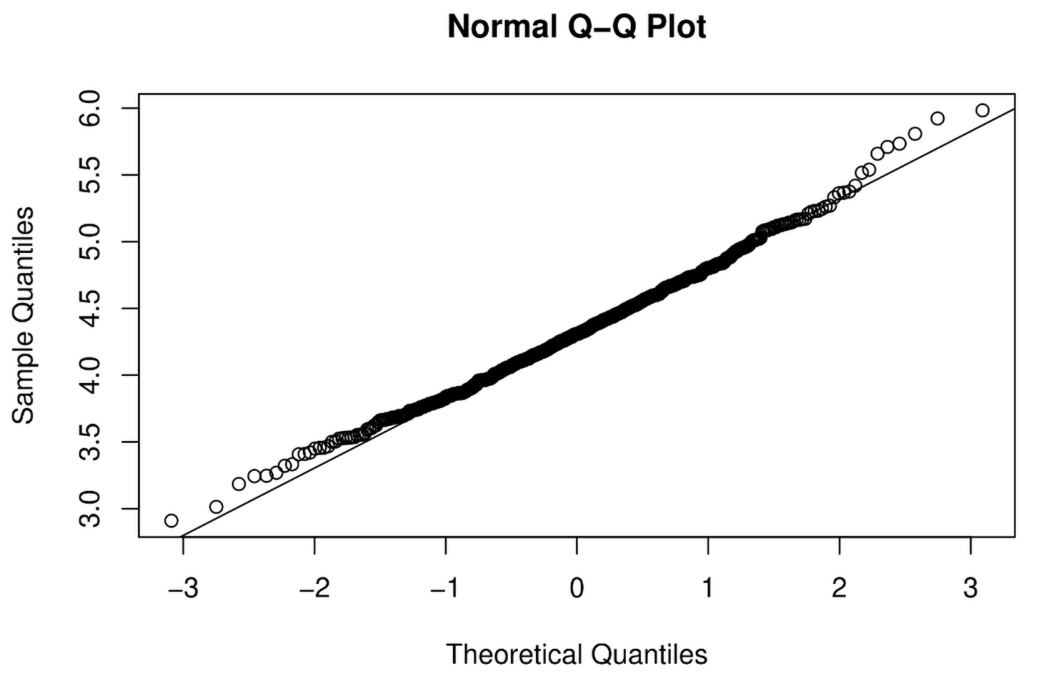
\includegraphics[height = 0.4\textwidth]{wind_qqplot_xbar}


\end{frame}

% =================================================
\section{Workshop 2: Seasonal Wind Speed}
% =================================================
\begin{frame}{Motivation}
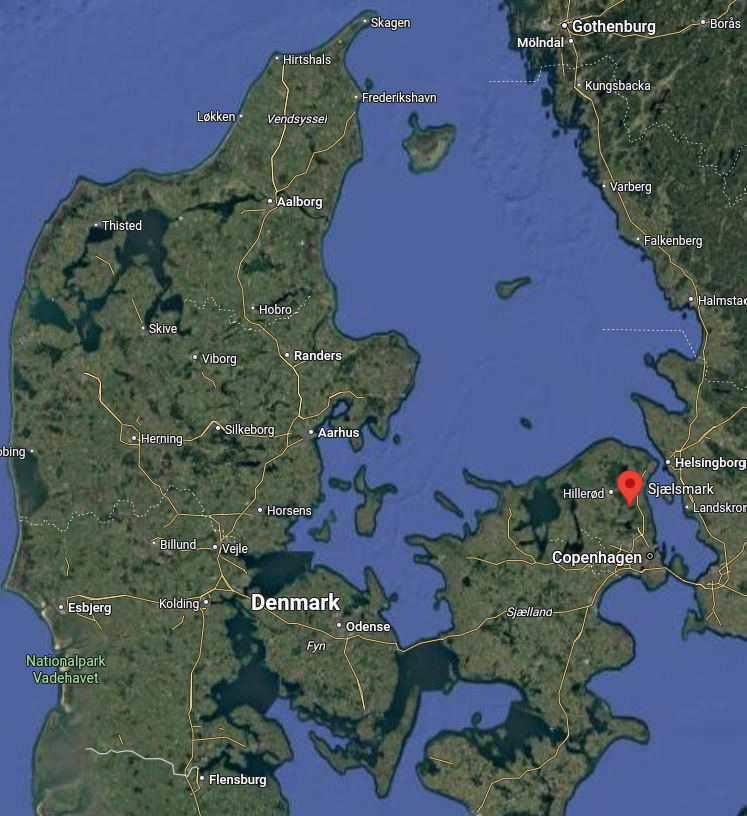
\includegraphics[width = 0.5\textwidth]{wind_location}

\end{frame}
% -------------------------------------------------
\begin{frame}{Seasonal Wind Speed Data}
Quarterly average wind speeds (2001--2019) at Sj\ae lsmark, Denmark:

\[
\text{quarters: } \text{spring, summer, autumn, winter}
\]

\begin{itemize}
  \item Assumption: Quarterly averages $\approx$ Normal (CLT)
  \item Significance level: $\alpha = 0.05$
\end{itemize}

\end{frame}

% -------------------------------------------------
\begin{frame}{Comparison of Spring and Autumn: Variances}
Null hypothesis:
\[
H_0: \sigma_{\text{spring}}^2 = \sigma_{\text{autumn}}^2, \quad
H_A: \sigma_{\text{spring}}^2 \neq \sigma_{\text{autumn}}^2
\]

\begin{itemize}
  \item F-test statistic: $F = s_{\text{spring}}^2 / s_{\text{autumn}}^2$
  \item Degrees of freedom: $df_{\text{spring}} = n_{\text{spring}}-1$, $df_{\text{autumn}} = n_{\text{autumn}}-1 \Rightarrow df=18$
  \item Two-sided p-value: $0.704 \Rightarrow$ do not reject $H_0 \Rightarrow$ We can assume
the variances in spring and autumn are approximately equal.
\end{itemize}

\end{frame}

% -------------------------------------------------
\begin{frame}{Comparison of Spring and Autumn: Means}
Null hypothesis:
\[
H_0: \mu_{\text{spring}} = \mu_{\text{autumn}}, \quad
H_A: \mu_{\text{spring}} \neq \mu_{\text{autumn}}
\]

\begin{itemize}
  \item Pooled standard deviation:
  \[
  s_p = \sqrt{\frac{(n_{\text{spring}}-1)s_{\text{spring}}^2 + (n_{\text{autumn}}-1)s_{\text{autumn}}^2}{n_{\text{spring}}+n_{\text{autumn}}-2}}
  \]
  \item Standard error: $SE = s_p \sqrt{\frac{1}{n_{\text{spring}}} + \frac{1}{n_{\text{autumn}}}}$
  \item t-statistic: $t = (\bar x_{\text{spring}} - \bar x_{\text{autumn}})/SE$
  \item p-value: $0.0059 < 0.05 \Rightarrow$ reject $H_0 \Rightarrow $ The difference in means is statistically significant.
\end{itemize}

\end{frame}

% -------------------------------------------------
\begin{frame}{Comparison of Spring and Autumn: Means}
\[
CI = (\bar x_{\text{spring}} - \bar x_{\text{autumn}}) \pm t_{1-\alpha/2, df} \cdot SE
\]

\[
CI = [0.077, 0.427]
\]

\begin{itemize}
  \item Spring winds significantly higher than autumn
  \item Interpretation: 95\% confident that the difference in means is positive
\end{itemize}
\end{frame}

% -------------------------------------------------
\begin{frame}{Boxplots of Quarterly Wind Speeds}
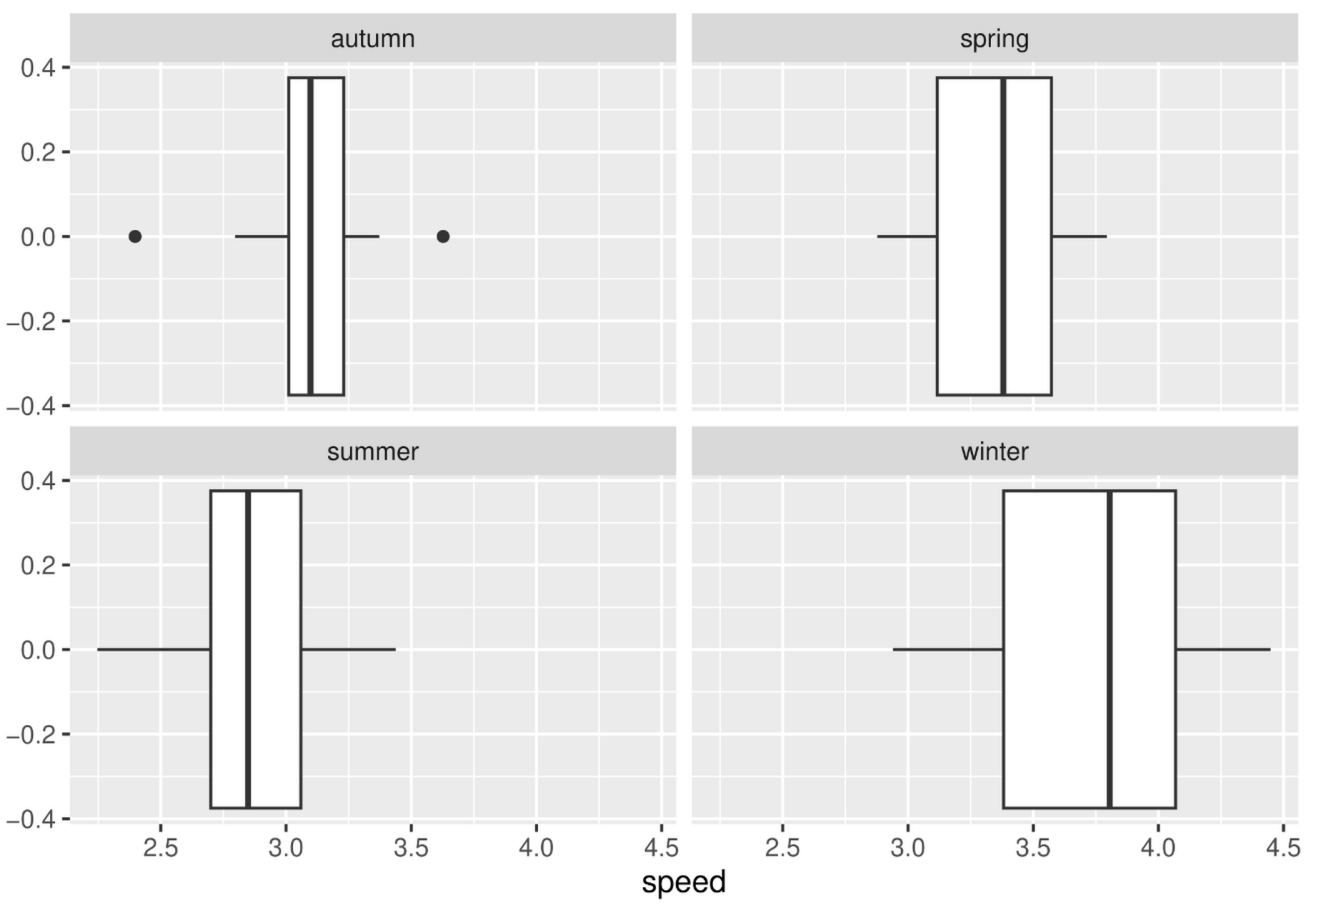
\includegraphics[width=0.6\textwidth]{wind_boxplot}

\begin{itemize}
  \item Box: Q1 to Q3, median line at Q2
  \item Whiskers: $[Q1-1.5\cdot IQR, Q3+1.5\cdot IQR]$
  \item Outliers shown as dots
  \item Winter shows highest median, summer the lowest
\end{itemize}

\end{frame}

% -------------------------------------------------
\begin{frame}{Testing Differences Across All Quarters}
Null hypothesis:
\[
H_0: \mu_{\text{spring}} = \mu_{\text{summer}} = \mu_{\text{autumn}} = \mu_{\text{winter}}
\]

\begin{itemize}
  \item Model: $speed \sim quarter$
  \item F-test: p-value $< 0.001 \Rightarrow$ reject $H_0 \Rightarrow$ the difference in means is statistically significant. 
  \item Multiple R-squared: 0.52 $\to$ 52\% of total variability explained by quarter
\end{itemize}
\end{frame}

% -------------------------------------------------
\begin{frame}{Tukey's Test}
Tukey test adjusts for multiple testing:

\begin{itemize}
  \item Winter > all other quarters (all p-values $\ll 0.05$)
  \item Summer vs spring: spring significantly higher
  \item Spring-autumn and summer-autumn: not significant after adjustment
\end{itemize}

\begin{itemize}
  \item CI for spring-autumn difference (Tukey): $[-0.012, 0.516]$  
    \begin{itemize}
      \item Wider than t-test CI, includes 0
      \item Multiple comparison adjustment reduces significance
  \end{itemize}
\end{itemize}
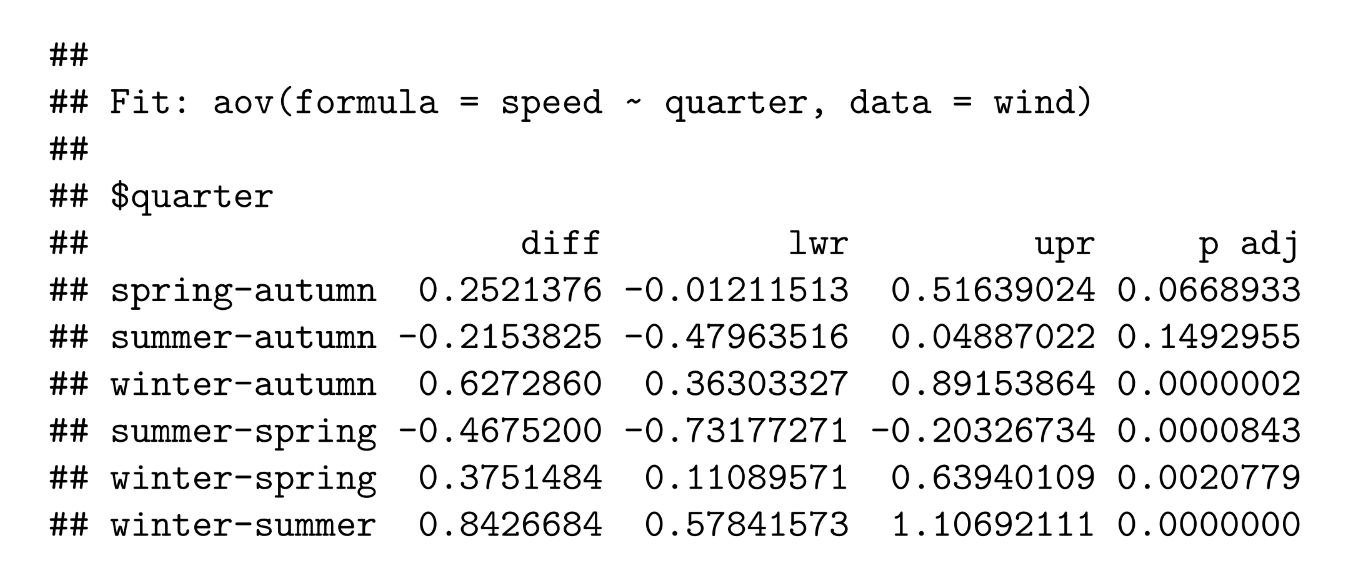
\includegraphics[height = 0.3\textwidth]{wind_tuckey}

\end{frame}


% =================================================
\section{Workshop 3: Battery Capacity}
% =================================================

% -------------------------------------------------
\begin{frame}{Battery Capacity Data}
We study battery capacity loss $Q$ measured at different temperatures.

\begin{itemize}
  \item Response variable: capacity loss $Q$ (in \%)
  \item Predictors:
  \begin{itemize}
    \item Number of charge cycles (FEC)
    \item Temperature: $35^\circ$, $40^\circ$, $45^\circ$ C
  \end{itemize}
  \item Log-transformed variables:
  \[
  \log(Q), \quad \log(\text{FEC})
  \]
\end{itemize}

\begin{itemize}
  \item Temperature treated as a categorical variable
\end{itemize}

\end{frame}

% -------------------------------------------------
\begin{frame}{Exploratory Analysis}
Scatter plot of $\log(Q)$ versus $\log(\text{FEC})$ colored by temperature.

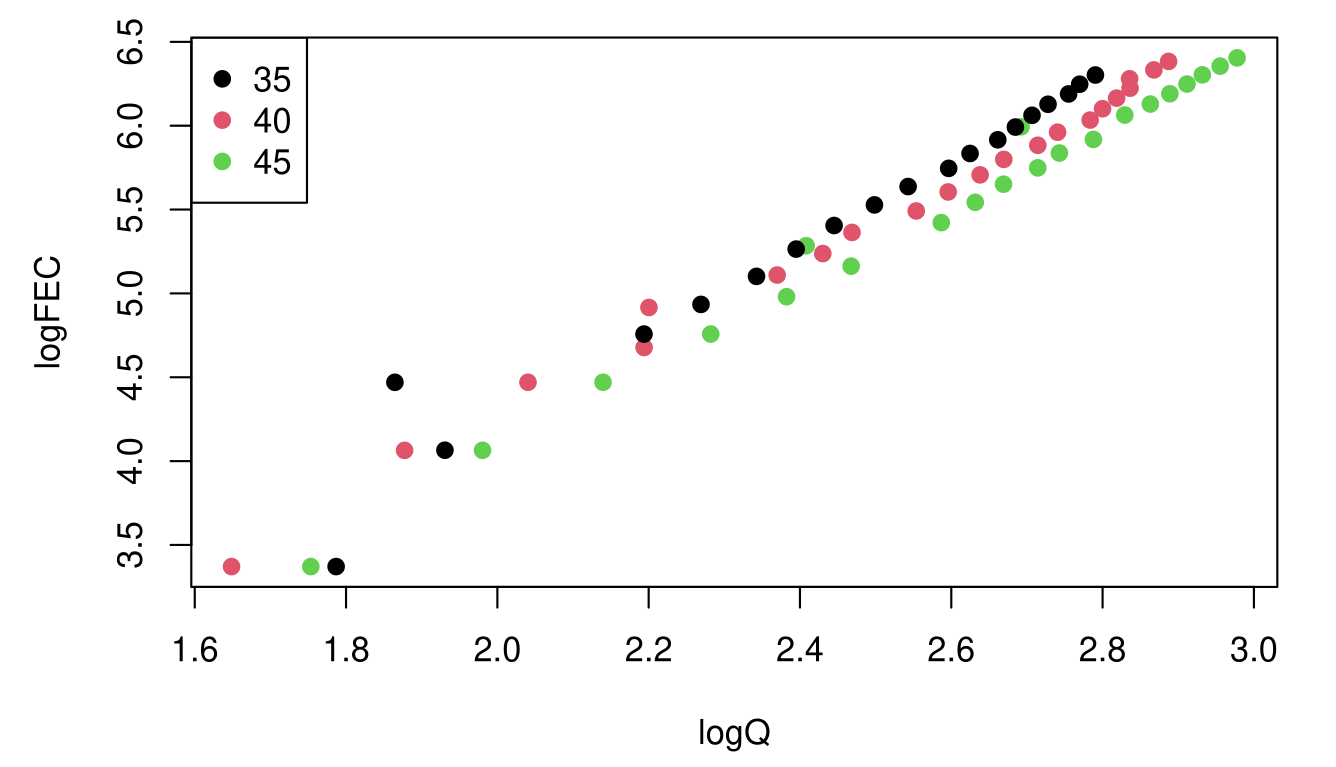
\includegraphics[width=0.65\textwidth]{battery_scatter}

\begin{itemize}
  \item Strong linear relationship
  \item Higher temperatures shift the relationship
\end{itemize}

\end{frame}

% -------------------------------------------------
\begin{frame}{Correlation Analysis}
Correlation between $\log(Q)$ and $\log(\text{FEC})$ for each temperature:

\[
r_{35} = 0.98, \quad
r_{40} = 0.997, \quad
r_{45} = 0.994
\]

\begin{itemize}
  \item Correlation measures strength of linear dependence
  \item Values close to 1 indicate very strong linear association
  \item Confirms visual impression from the scatter plot
\end{itemize}

\end{frame}

% -------------------------------------------------
\begin{frame}{Multiple Regression Model (No Interaction)}
We consider the model:
\[
\log(Q_i) =
\beta_0
+ \beta_1 \log(\text{FEC}_i)
+ \beta_2 \mathbb{I}(T_i = 40)
+ \beta_3 \mathbb{I}(T_i = 45)
+ \varepsilon
\]

\begin{itemize}
  \item $\alpha$: intercept
  \item $\beta_1$: effect of charge cycles at 35C
  \item $\beta_2$: effect of 40C
  \item $\beta_3$: effect of 45C
  \item $\varepsilon \sim N(0,\sigma^2)$
\end{itemize}

\end{frame}

% -------------------------------------------------
\begin{frame}{Estimated Regression Model}
Estimated model:
\[
\log(Q_i) =
0.224846
+ 0.411014 \log(\text{FEC}_i)
+ 0.043310 \mathbb{I}(T_i = 40)
+ 0.106577 \mathbb{I}(T_i = 45)
+ \varepsilon_i
\]

\begin{itemize}
  \item $\log(\text{FEC})$ has a strong positive effect
  \item Higher temperatures increase capacity loss
  \item Predictors are statistically significant
\end{itemize}

\end{frame}

% -------------------------------------------------
\begin{frame}{Inference and Model Fit}
\begin{itemize}
  \item t-statistics computed as:
  \[
  t = \frac{\text{Estimate}}{\text{Std. Error}}
  \]
  \item The amount of std. errors away each coefficient is from 0
\end{itemize}

\begin{itemize}
  \item Multiple $R^2 = 0.982$
  \item Interpretation:
  \item 98\% of the variability in $\log(Q)$ is explained
\end{itemize}

\end{frame}

% -------------------------------------------------
\begin{frame}{Overall F-Test}
Null hypothesis:
\[
H_0: \beta_1 = \beta_2 = 0
\]

\begin{itemize}
  \item F-test compares explained to unexplained variance
  \item p-value $< 0.001$
  \item Reject $H_0$
\end{itemize}

\begin{itemize}
  \item At least one predictor significantly affects $\log(Q)$
\end{itemize}

\end{frame}

% -------------------------------------------------
\begin{frame}{Interaction Model}
We test whether temperature modifies the effect of charge cycles:
\[
\log(Q_i) =
\beta_0
+ \beta_1 \log(\text{FEC}_i)
+ \beta_2 \mathbb{I}(T_i = 40)
+ \beta_3 \mathbb{I}(T_i = 45)
\]
\[
+ \beta_4 \log(\text{FEC}_i)\mathbb{I}(T_i = 40)
+ \beta_5 \log(\text{FEC}_i)\mathbb{I}(T_i = 45)
+ \varepsilon_i
\]

\begin{itemize}
  \item Compare models with and without interaction
  \item F-test: $p = 0.13$
\end{itemize}

\begin{itemize}
  \item No significant interaction
\end{itemize}

\end{frame}

% -------------------------------------------------
\begin{frame}{Model Fits}
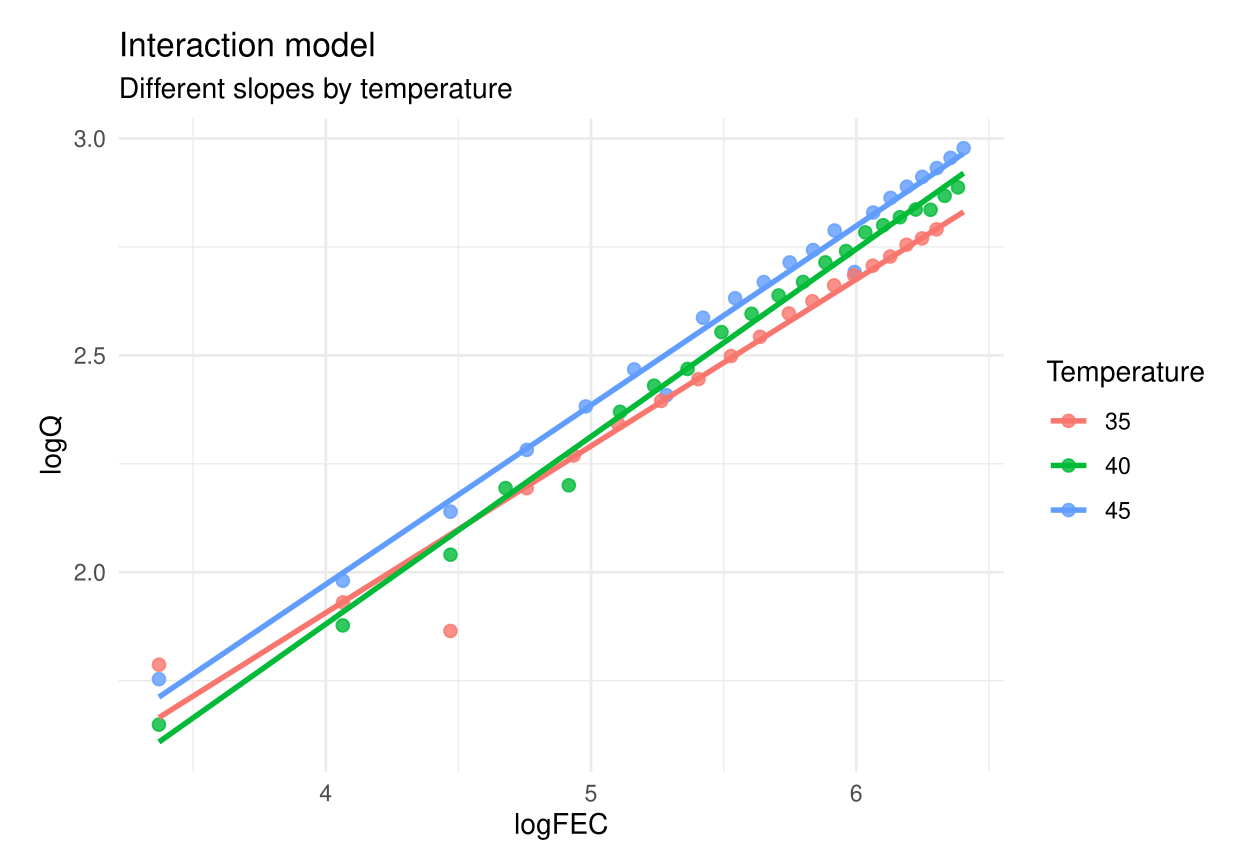
\includegraphics[width=0.48\textwidth]{battery_fit_1}
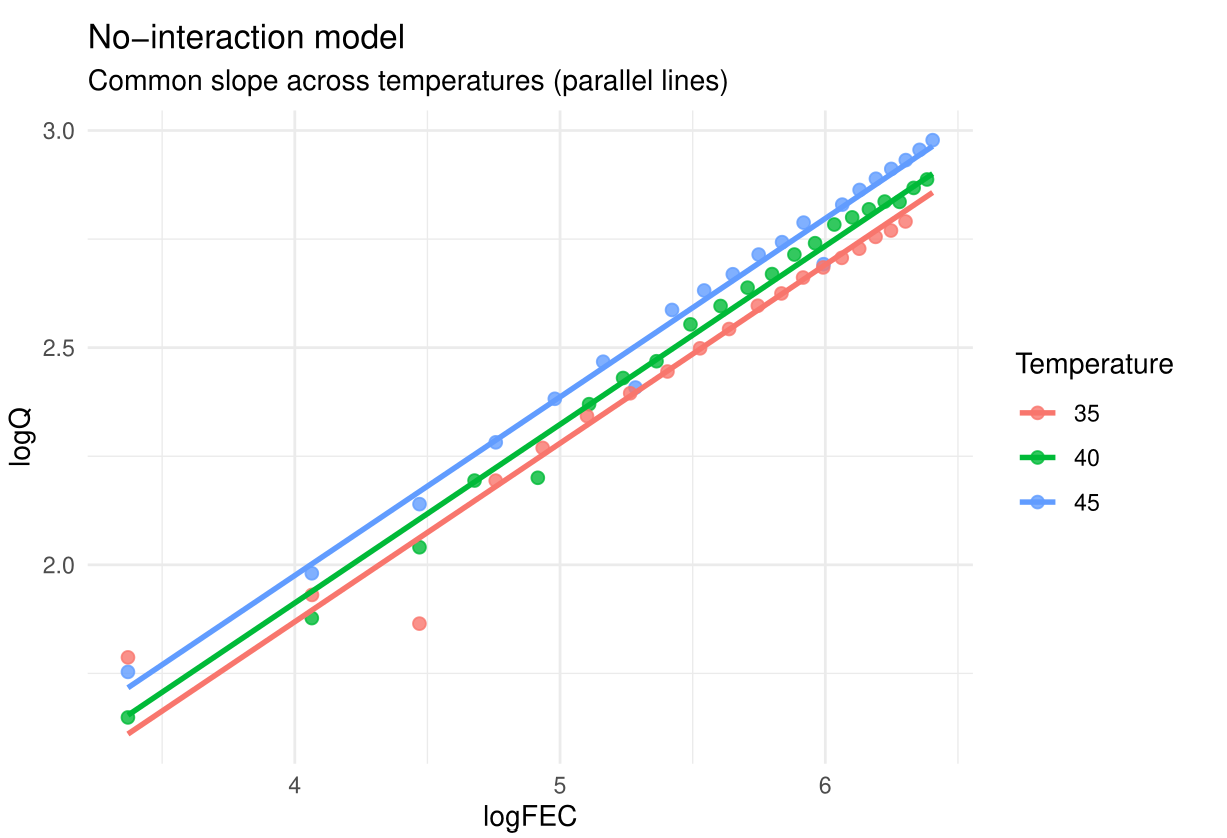
\includegraphics[width=0.48\textwidth]{battery_fit_2}


\end{frame}

% -------------------------------------------------
\begin{frame}{Residual Analysis}
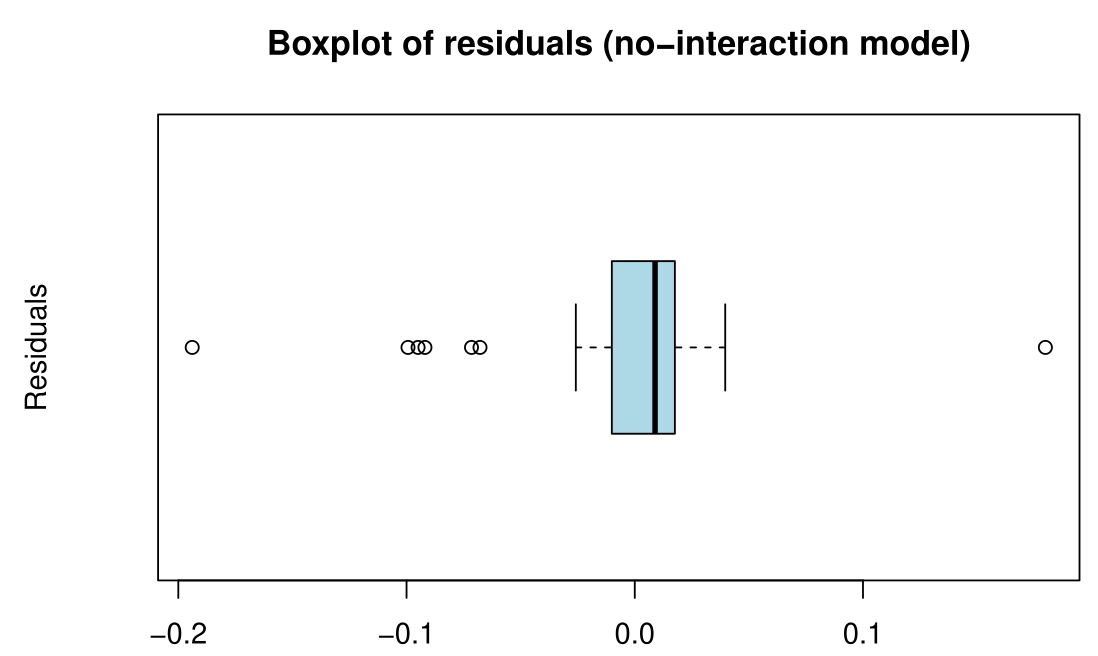
\includegraphics[width=0.6\textwidth]{battery_residuals}

\begin{itemize}
  \item Median residual close to zero
  \item Indicates unbiased predictions
  \item Some outliers present
\end{itemize}

\end{frame}

% -------------------------------------------------
\begin{frame}{Conclusions}
\begin{itemize}
  \item Battery capacity loss increases with:
  \begin{itemize}
    \item Number of charge cycles
    \item Temperature
  \end{itemize}
  \item Linear regression explains most variability
  \item No evidence of interaction between predictors
\end{itemize}

\end{frame}


% =================================================

\section{Workshop 4: DC Motor Model}

% -------------------------------------------------
\begin{frame}{Problem: DC Motor}
\begin{itemize}
  \item Input-output time series
  \item Noise and disturbances
  \item Goal: Model motor velocity as a function of input voltage
\end{itemize}

\begin{center}
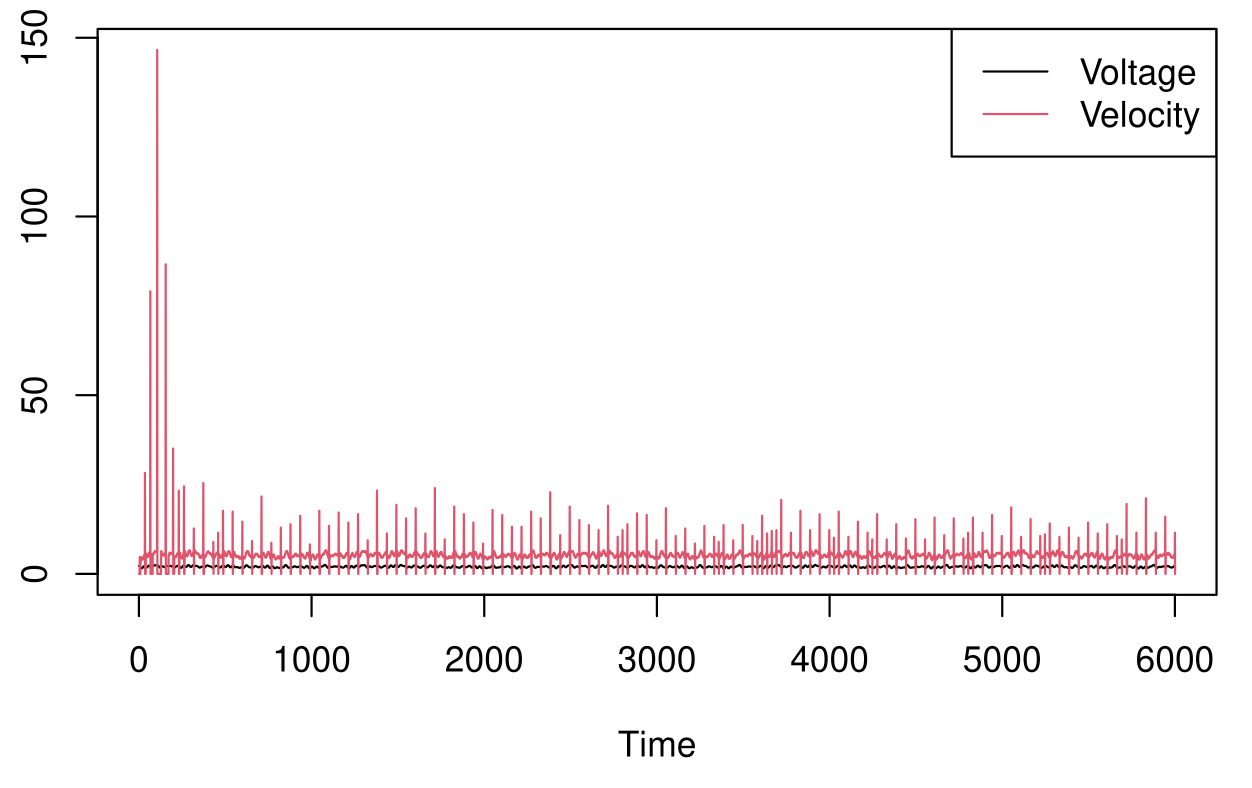
\includegraphics[width=0.6\textwidth]{motor_timeseries_full}
\end{center}
\end{frame}

% -------------------------------------------------
\begin{frame}{Data Visualization and Cleaning}
\begin{itemize}
  \item Raw data: voltage (V) and motor velocity (rad/s)
  \item Sampling time: 0.01 s
  \item Zoom-in reveals noise and periodic disturbances
  \item Data cleaning:
  \begin{itemize}
    \item Remove first 500 samples
    \item Set velocities outside $[3,7]$ rad/s to NA
    \item Pick interval $t = 1000:2000$ for analysis
  \end{itemize}
\end{itemize}

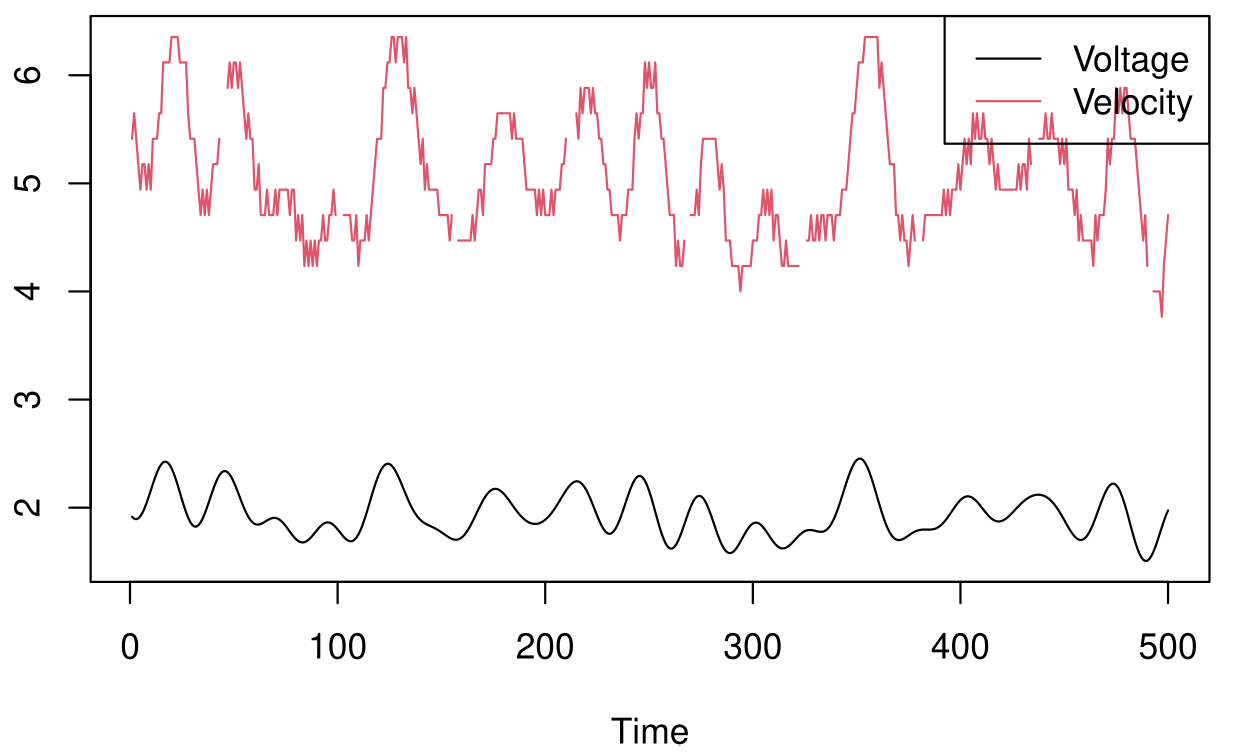
\includegraphics[width=0.6\textwidth]{motor_timeseries_adj}
\end{frame}

% -------------------------------------------------
\begin{frame}{Cross-Correlation Function (CCF)}
\begin{itemize}
  \item Detect delay between input voltage and output velocity
  \item CCF peak indicates system delay
  \item Maximum correlation → estimated lag: -5 samples
  \item Sampling time = 0.01 s → delay = -0.05 s
\end{itemize}

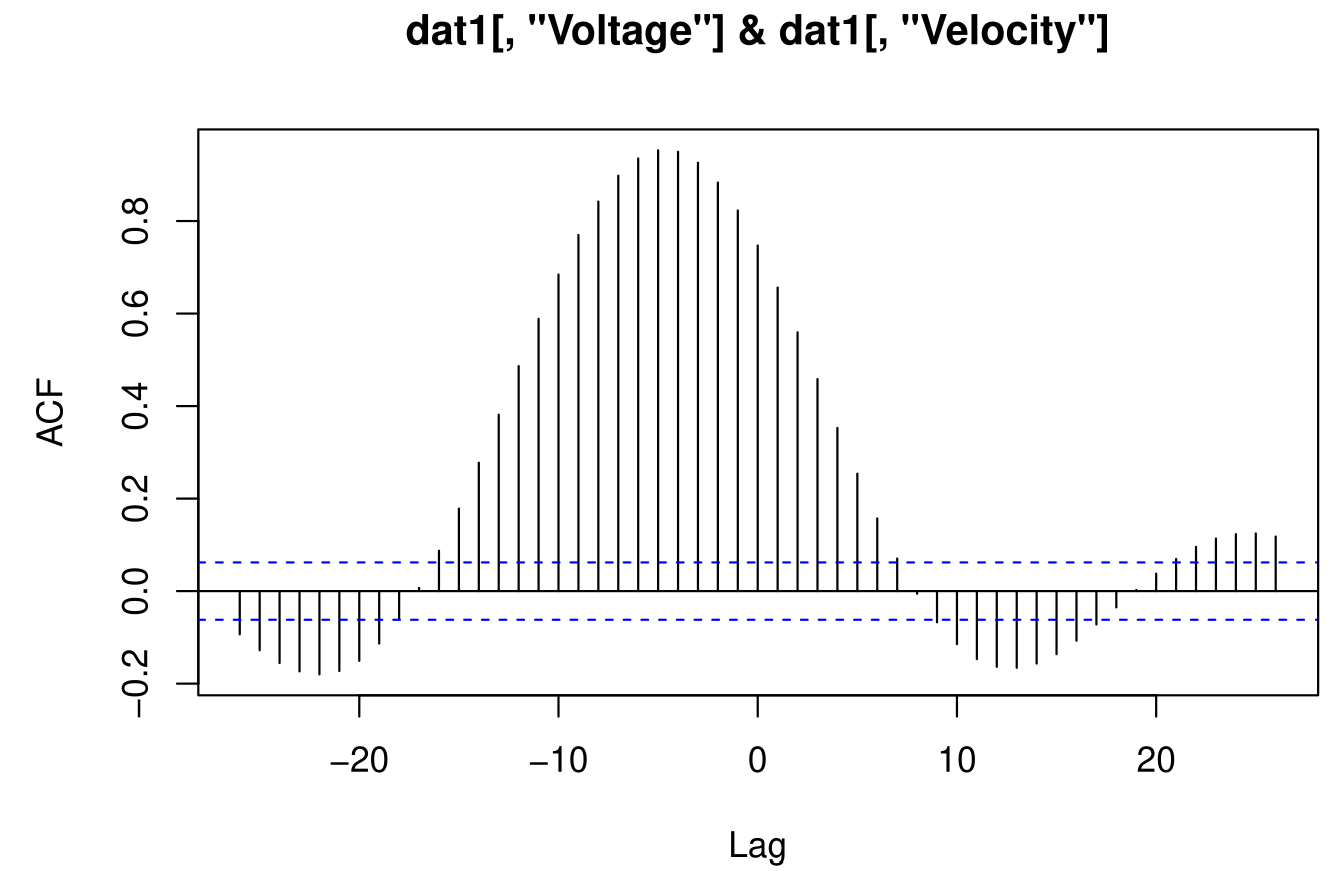
\includegraphics[width=0.6\textwidth]{motor_lag}
\end{frame}

% -------------------------------------------------
\begin{frame}{Linear Regression with AR(1) Noise}
\[
\omega_t = \beta_0 + \beta_1 V_t + \alpha \epsilon_{t-1} + W_t
\]

\begin{itemize}
  \item Fit AR(1) model with input voltage as exogenous variable
  \item Estimated parameters:
  \[
  \beta_0 = 1.6348, \quad \beta_1 = 1.7945, \quad \alpha = 0.8584
  \]
  \item Noise ACF: $\rho(h) = \alpha^h = 0.8584^h$
\end{itemize}

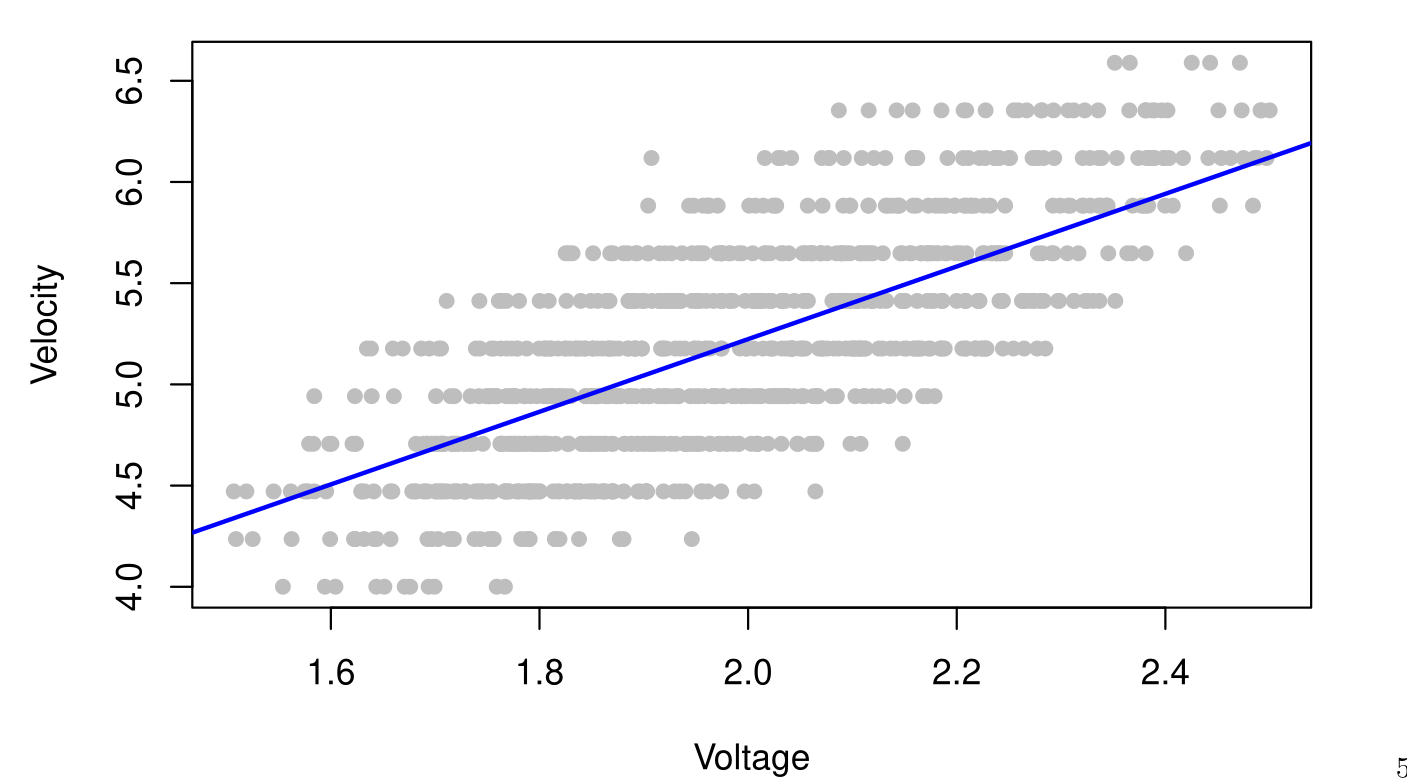
\includegraphics[width=0.6\textwidth]{motor_model_1}
\end{frame}

% -------------------------------------------------
\begin{frame}{Residual Analysis for AR(1) Model}
\begin{itemize}
  \item Residuals should resemble white noise
  \item Check time series plot and correlogram
  \item Some oscillations remain from original periodic disturbance
\end{itemize}

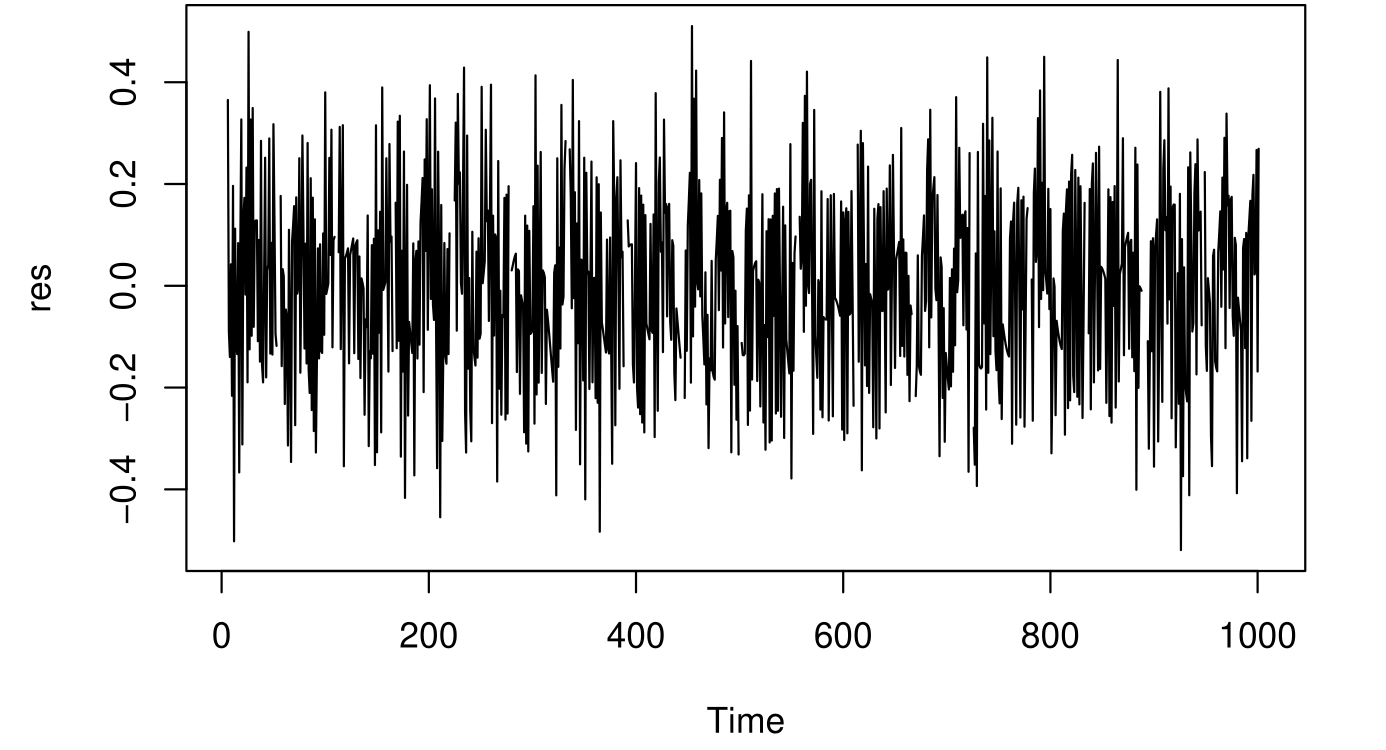
\includegraphics[width=0.48\textwidth]{motor_res_1}
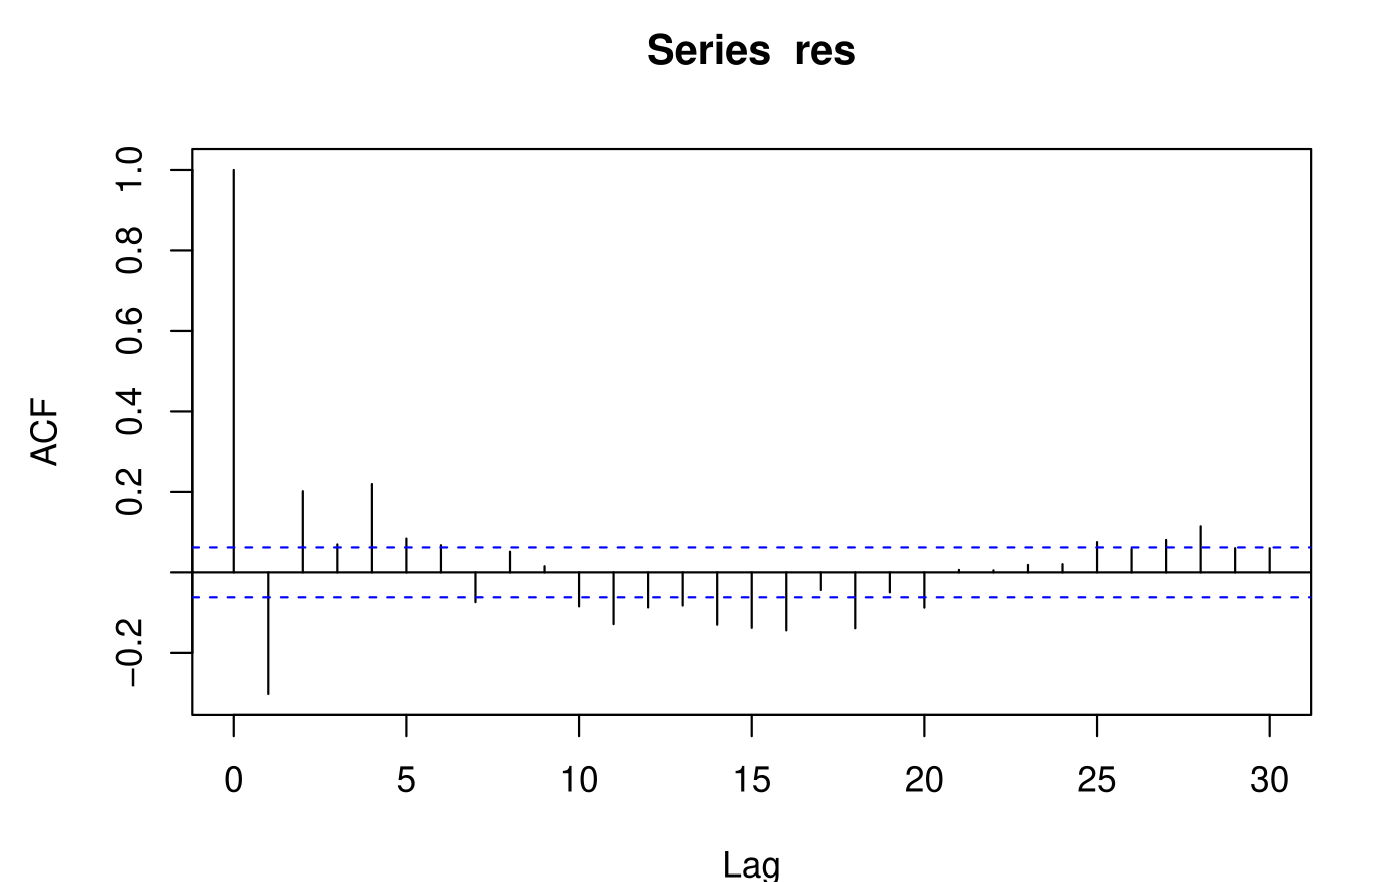
\includegraphics[width=0.48\textwidth]{motor_cor_1}
\end{frame}

% -------------------------------------------------
\begin{frame}{ARMA(p,q) Model Selection}
\begin{itemize}
  \item Fit ARMA(p,q) models with $p,q = 0,1,2,3$
  \item Compare using AIC
  \item Best model: ARMA(3,3) with lowest AIC
\end{itemize}

\[
\omega_t = \beta_0 + \beta_1 V_t + n_t, n_t = \sum_{i=1}^3 \phi_i n_{t-i} + \sum_{j=1}^3 \theta_j \epsilon_{t-j} + \epsilon_t
\]

\[
\omega_t = 0.4916 + 2.3687 V_t + n_t
\]

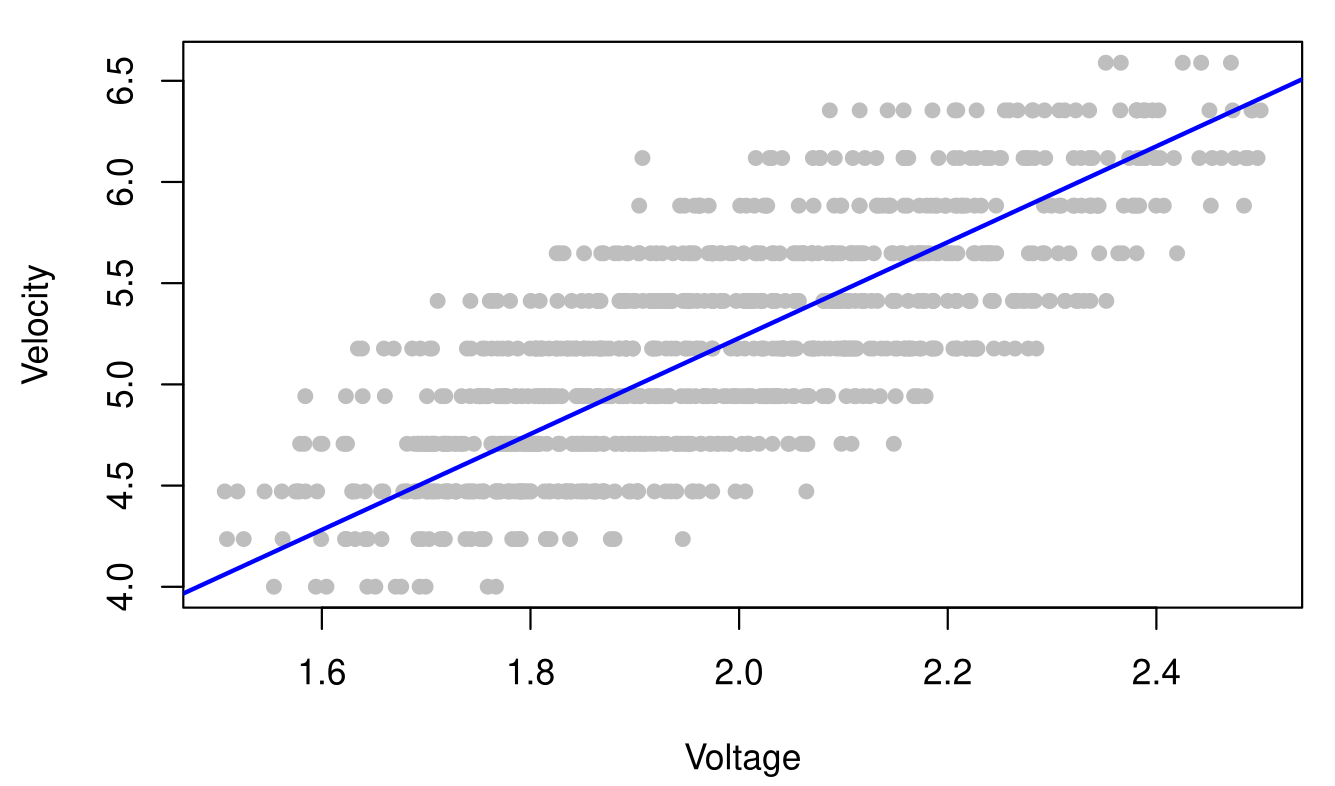
\includegraphics[width=0.6\textwidth]{motor_model_2}

\end{frame}

% -------------------------------------------------
\begin{frame}{ARMA(3,3) Residuals}
\begin{itemize}
  \item Residuals checked for whiteness
  \item Correlogram confirms good fit
\end{itemize}

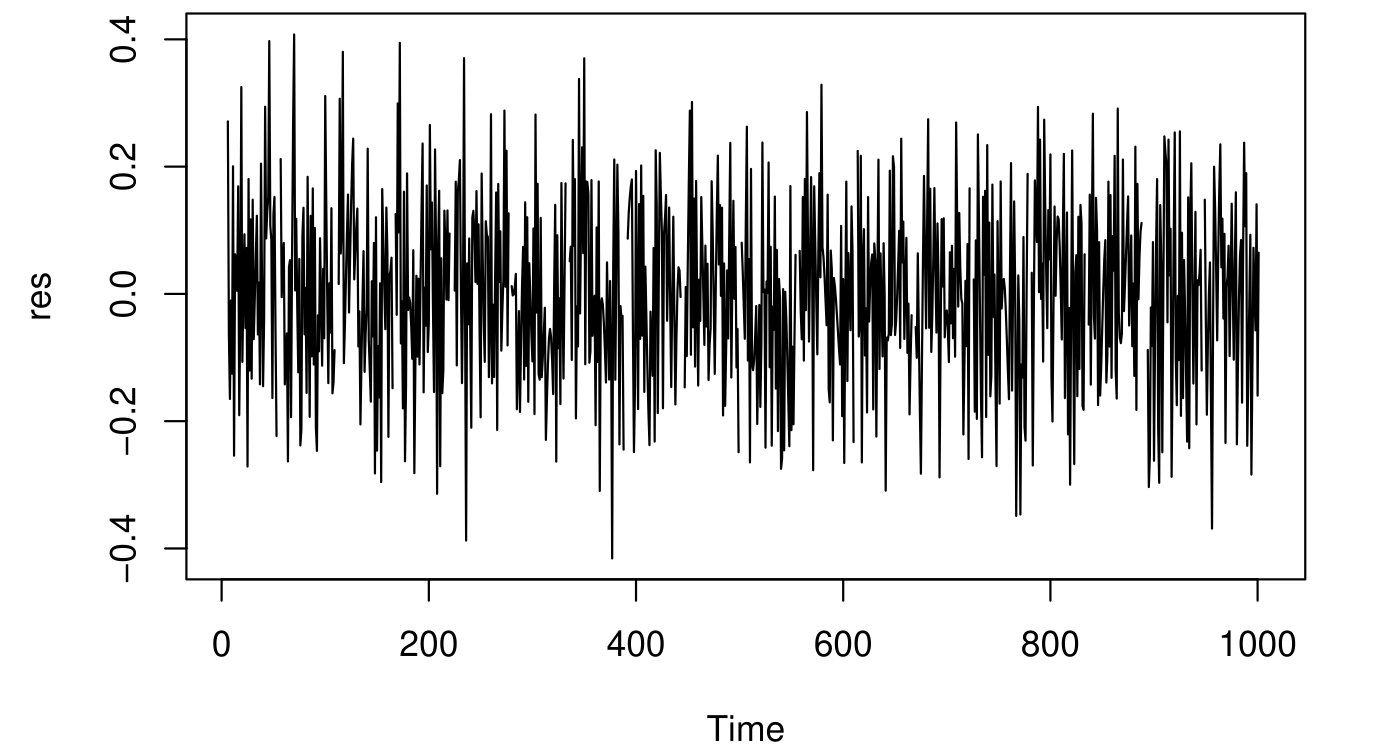
\includegraphics[width=0.48\textwidth]{motor_res_2}
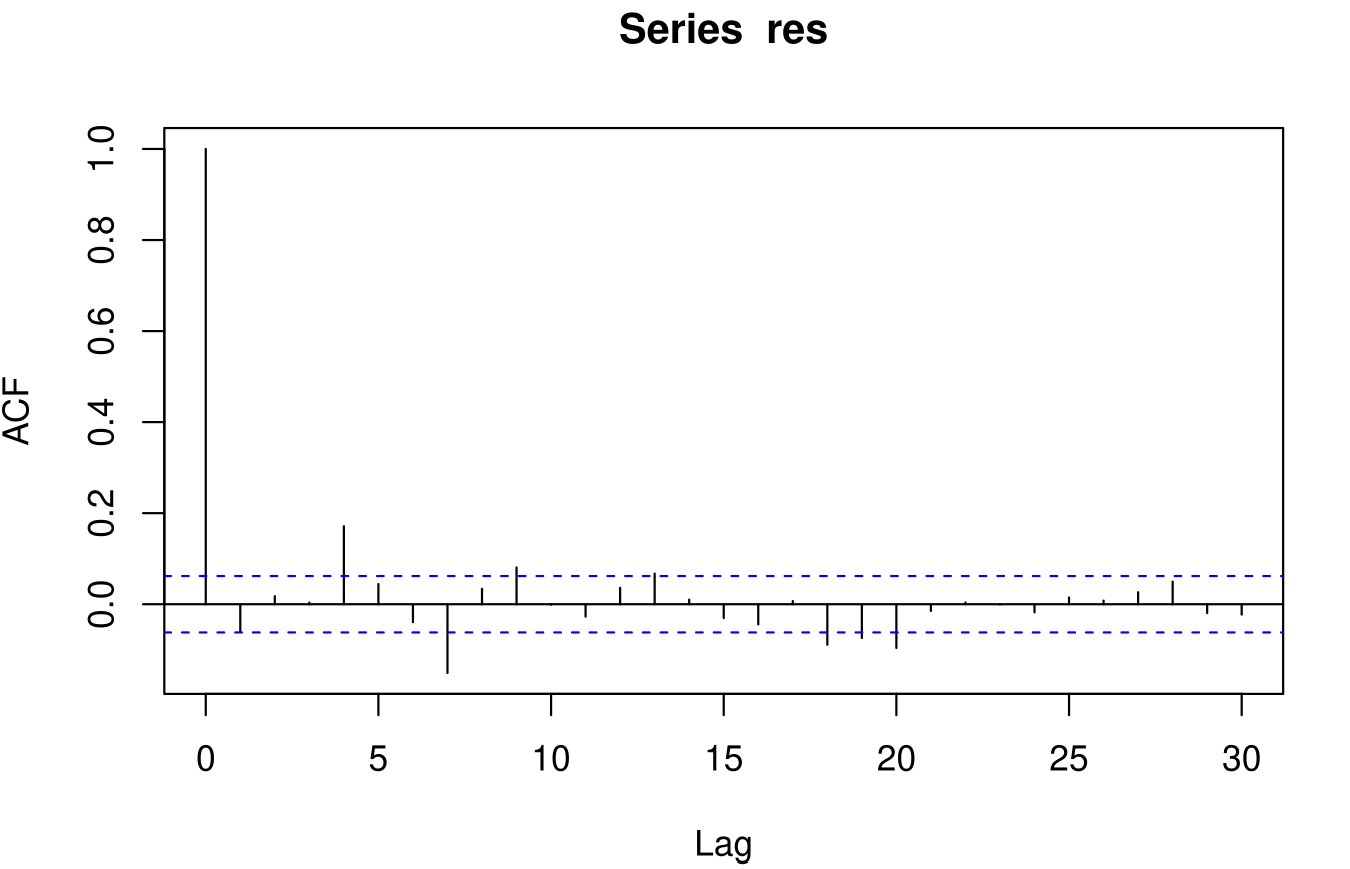
\includegraphics[width=0.48\textwidth]{motor_cor_2}
\end{frame}

% -------------------------------------------------
\begin{frame}{Regression Slope and Confidence Interval}
\begin{itemize}
  \item Estimated slope: $\beta_1 = 2.3687$
  \item 95\% CI: $[2.145 , 2.592]$
  \item Graphical visualization:

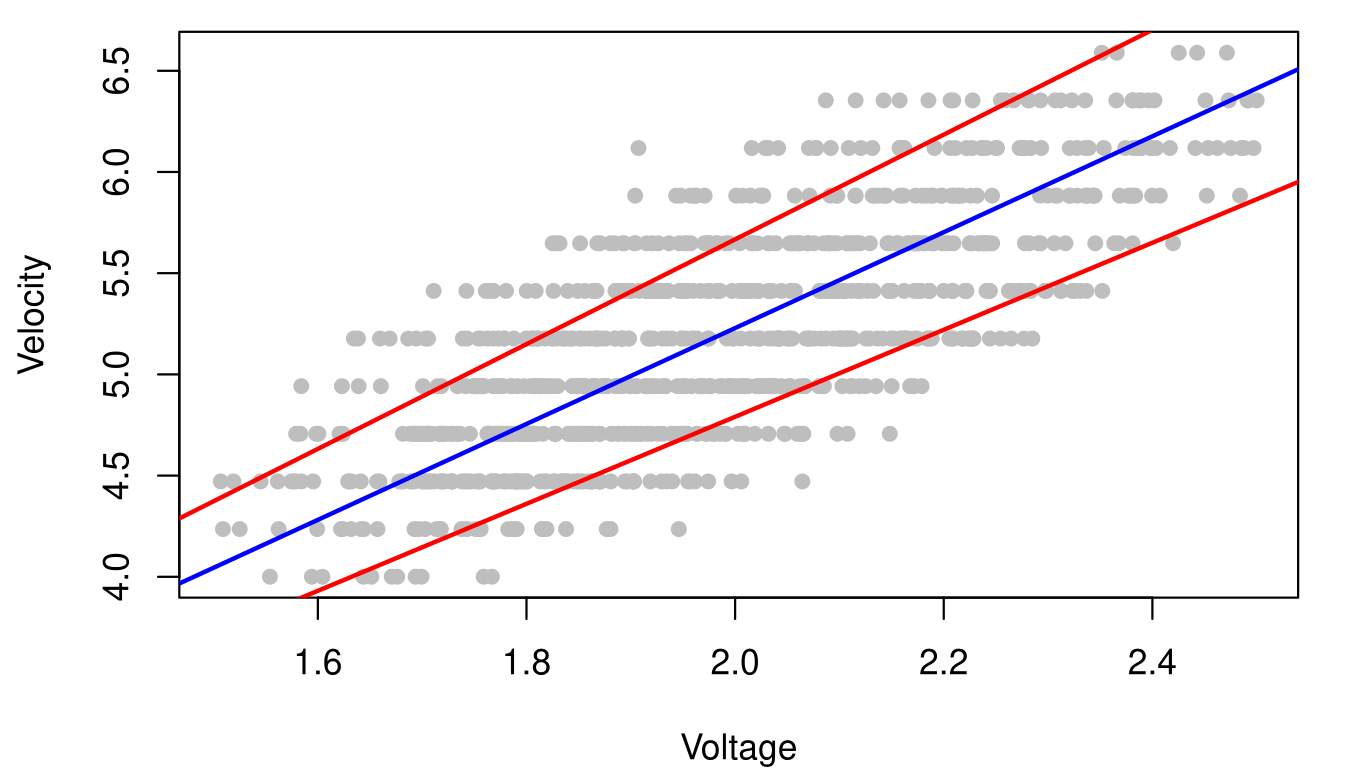
\includegraphics[width=0.6\textwidth]{motor_model_2_conf}
\end{itemize}
\end{frame}

% -------------------------------------------------
\begin{frame}{Prediction Example}
\begin{itemize}
  \item Next voltage: $V = 2.23$
  \item Predicted velocity: $\hat{\omega} = 5.8535$ rad/s
  \item 95\% prediction interval: $[5.539 , 6.168]$ rad/s
\end{itemize}

\end{frame}

% -------------------------------------------------

\end{document}
